%\documentclass[a4paper,twocolumn]{article}
\documentclass[a4paper,11pt]{article}
% \usepackage[left=3.8cm,right=3.8cm]{geometry}
\usepackage[latin1]{inputenc}
% \usepackage{amsmath}
% \usepackage[dvips]{graphics}
\usepackage{graphicx}
\usepackage{color}
\usepackage{url}
% \usepackage{draftcopy}
% \usepackage{subfigure}
% \usepackage{epsfig}
% \usepackage{hthtml}
\usepackage{ifthen}
\usepackage{listings}
\usepackage{makeidx}

\usepackage[english]{babel}
\selectlanguage{english}

\makeindex

\newcommand{\teseoversion}[0]{2.0.16}
% \newcommand{\turnseismograms}[0]{{{\color{red}T}urn the {\color{red}E}ldest {\color{red}S}eismograms into the {\color{red}E}lectronic {\color{red}O}riginal {\color{red}O}nes}}
\newcommand{\turnseismograms}[0]{{{\bfseries T}urn the {\bfseries E}ldest {\bfseries S}eismograms into the {\bfseries E}lectronic {\bfseries O}riginal {\bfseries O}nes}}

%%%%%%%%%%%%%%%%%%%%%%%%%%%%%%%%%%%%
% printOut default is "html"
\newcommand{\teseo}[0]{{Teseo\small 2}}
\newcommand{\teseoscalegraphics}[0]{1}
\newcommand{\teseoprequote}[0]{''}
\newcommand{\teseohyphen}[0]{---}

% printOut can be "paper"
\newcommand{\printOut}[1]
{
  \ifthenelse{\equal{#1}{paper}}{
% Paper format
	  \renewcommand{\teseo}[0]{{Teseo\small$^2$}}
	  \renewcommand{\teseoscalegraphics}[0]{0.5}
	  \renewcommand{\teseoprequote}[0]{``}
	  \renewcommand{\teseohyphen}[0]{$- -$}
}{}
}

\printOut{paper}

%%%%%%%%%%%%%%%%%%%%%%%%%%%%%%%%%%%%
\newcommand{\teseoquote}[1]{\teseoprequote#1''}
\newcommand{\teseoincludegraphics}[2]{ \includegraphics[scale=#1]{#2} }

\newcommand{\teseolearn}[0]{{\bfseries TeseoLearn}}
\newcommand{\gimp}[0]{{GIMP}\index{GIMP}}
\newcommand{\sismos}[0]{{\bfseries Sismos}}
\newcommand{\beziername}[0]{B\'ezier}

\newcommand{\parolachiave}[1]{{\bfseries \itshape #1}\index{Keywords!#1}}
\newcommand{\prototipo}[1]{{\emph{#1}}\index{Prototype!#1}}

\newcommand{\tabname}[1]{{\itshape #1}\index{Tabs!#1}}
\newcommand{\menuname}[1]{{\itshape \bfseries #1}\index{Menu!#1}}
\newcommand{\fileformat}[1]{{\itshape #1}\index{File formats!#1}}
\newcommand{\xcf}[0]{\fileformat{xcf}}
\newcommand{\parameter}[1]{{\itshape #1}\index{Parameters!#1}}
\newcommand{\button}[1]{{\itshape #1}\index{Buttons!#1}}
\newcommand{\filter}[1]{{\itshape #1}\index{Filters!#1}}
\newcommand{\gimptool}[1]{{\itshape #1}\index{GIMP tools!#1}}
\newcommand{\teseooperations}[1]{{\itshape #1}\index{Teseo operations!#1}}
\newcommand{\teseomodule}[1]{{\itshape #1}\index{Teseo modules!#1}}
\newcommand{\softwaredevel}[1]{{\itshape #1}\index{Software development!#1}}
\newcommand{\gtk}[0]{\softwaredevel{GTK+}\index{GTK+}}
\newcommand{\gtkdatabox}[0]{\softwaredevel{GtkDataBox}}
\newcommand{\glib}[0]{\softwaredevel{GLib}\index{GLib}}
\newcommand{\cvsrevision}[0]{$ $Revision: 1.63 $ $}
\newcommand{\cvsdate}[0]{$ $Date: 2007/04/13 07:02:00 $ $}
\newcommand{\cvsrevisiondate}[0]{\cvsrevision  --  \cvsdate}

\newcommand{\smallmarginpar}[1]{\marginpar{\footnotesize{#1}}}
% \newcommand{\todo}[1]{ \smallmarginpar{{\bfseries TO DO} {\small #1}}}
\newcommand{\todo}[1]{

{\color{red}
{\bfseries TO DO:} #1
}

}


\newcommand{\subtitle}[1]{

\vspace{0.25cm}
\begin{center}
{\bfseries #1}
\end{center}

}

\title{
  {\bfseries \teseo\ User Manual} \\
  {\footnotesize \turnseismograms\ -- \teseoversion}
}

\author{
  {\bfseries Stefano Pintore, Matteo Quintiliani} \\
  {\small \itshape Istituto Nazionale di Geofisica e Vulcanologia, Roma, Italy}
}

\date{}

\makeatletter 
\newcommand{\listofwarnings}{
\section{Warnings}

In this section are resumed all warnings contained in the manual.

%\begin{itemize}
\vspace{0.3cm}
\@starttoc{low}
% \end{itemize}
} 
\newcommand{\warning}[1]{

{\bfseries \itshape {\color{red}Warning}}: #1 \addcontentsline{low}{warning}{#1}


} 
\newcommand{\l@warning}[2]{
% \item #1 ({\itshape pag. #2})
\par\noindent $\bullet$  #1 ({\itshape pag. #2})
\vspace{0.3cm}
}
\makeatother

% Tutti i listati saranno esempi  nel linguaggio C o C++
\lstset{language=C,basicstyle=\scriptsize}



\begin{document}

\maketitle

\begin{center}
* * * \\
This documentation needs further updates. \\
{\itshape \cvsrevisiondate} \\
Please, check last revision at \url{http://sismos.ingv.it/teseo/} \\
\end{center}

\tableofcontents

\newpage

\section{Introduction}

This document is the user manual of \teseo\ software -- {\itshape Copyright \copyright\ 2005} -- Stefano Pintore, Matteo Quintiliani.
{\itshape \cvsrevisiondate.}

\teseo\ is a software tool for seismogram digitization/vectorization and it is developed in the framework of the Sismos project \cite{sismoseos} at Istituto Nazionale di Geofisica e Vulcanologia (Italy).
This name was inspired by the myth of Theseus and it is also an acronym for {\itshape \turnseismograms}.

\teseo\ is a plug--in for GIMP -- GNU Image Manipulation Program -- that extends its functionalities for seismological studies.  The \gimp\ is a multiplatform photo manipulation tool freely distributed. It works on many operating systems, in many languages.

\teseo\ allows primarily for: 

\begin{itemize}
\item additional operations on the vectorized trace (i.e. resampling and alignment) 
\item supervised vectorization algorithms (colour weighted mean) 
\item analysis after trace vectorization, such as curvature correction and time realignment 
\item trace import/export in several formats (such as \fileformat{SAC}, \fileformat{SVG}, \fileformat{DXF}, \fileformat{ASCII}, Timemarks distances). 
\end{itemize}

In order to keep track of the stages and parameters of a seismogram vectorization, \teseo\ is able to write this information into the image saved in \xcf\ format. 

\teseo\ is developed following the \teseoquote{Open--Source} philosophy and it is freely distributed under GPL license. It is cross--platform and the sources, the binaries for Linux, Windows and Mac OS X, are periodically updated on the Sismos web site. 


Official web site: {\itshape \url{http://sismos.ingv.it/teseo/}}

Developer e--mail: {\itshape \url{mailto:teseo@ingv.it}}

User mailing--list: {\itshape \url{mailto:teseo-user@yahoogroups.com}}

ML archive: {\itshape \url{http://groups.yahoo.com/group/teseo-user/}}


\section{Installing Teseo}

Before installing \teseo\ you need to install \gimp\ 2.2. \teseo\ has never been tested on \gimp\ 2.0.

Please refer to the official website at \url{http://www.gimp.org/}, user manual \cite{gimphelp} and books \cite{bunks}, \cite{kylander}, for any information about it.


\teseo\ is developed on Linux but binaries are also available for other platforms such as Windows and Mac OS X.
You can be able to compile \teseo\ on every system where \gimp\ has been successfully installed.
Sources and some binary distributions can be downloaded at the official web site, \url{http://sismos.ingv.it/teseo/}

In this manual we provide basic information to install \teseo\ plug-in. For specific information, please follow instructions contained in the INSTALL file for your distribution.


\subsection{Teseo from Source}

\teseo\ is mostly developed in C language, one library is written in Fortran. In order to compile \teseo\, you need \softwaredevel{gcc}, \softwaredevel{g77} and \softwaredevel{libg2c}.

In general, \teseo\ works with \gimp\ 2.2, although version 2.2.6 or newer is recommended.
We develop \teseo\ using \gtk\ and \glib.
\gtk\ is a library for creating graphical user interfaces.
\glib\ is a general-purpose utility library, which provides many useful data types, macros, type conversions, string utilities, file utilities, a main loop abstraction, and so on. The versions of \gtk\ and \glib\ are the same used by \gimp.

Moreover, \teseo\ use a \gtk\ widget called \gtkdatabox\
which has been designed to display large amounts of numerical data fast and easy.
Version greater than 0.4.0 is required.
Please, refer to the section \ref{sec:credits} for downloading and documentation about \gtkdatabox.

\teseo\ sources are subdivided into three separate modules: two libraries (\teseomodule{gtk--addons}, \teseomodule{newuoa}) and the \gimp\ plug-in (\teseomodule{teseo--2}).
Unpack the file teseo--2.x.x.tar.gz and compile the source modules following this order: \teseomodule{gtk--addons}, \teseomodule{newuoa} and \teseomodule{teseo--2}.
You can use the stardard command sequence:

{\itshape
\begin{tabular}{l}
./configure \\
make \\
make install
\end{tabular} 
}


For \teseomodule{teseo--2}, you should launch the configure script with the same {\itshape prefix} of gimp--2.2 and, optionally, set the {\itshape datadir}. For example, if gimp--2.2 is configured with {\itshape \teseohyphen prefix=/mydir}, you have to  use:

{\itshape
\begin{tabular}{l}
./configure \teseohyphen prefix=/mydir \teseohyphen datadir=/mydir/share/gimp/2.0
\end{tabular} 
}


\subsection{Teseo for Linux}

First of all, install \gimp. Version 2.2.6 or newer is recommended.

Unpack the binary distribution from teseo--2.x.x--bin--linux.tar.gz and run these commands to install \teseo:

{\itshape
\begin{tabular}{l}
cd teseo--2.x.x--bin--linux \\
./setup.sh linux
\end{tabular} 
}

setup.sh needs gimptool--2.0 included in \gimp\ distributions.

To uninstall run:

{\itshape
\begin{tabular}{l}
cd teseo--2.x.x-bin--linux \\
./setup.sh linuxuninstall
\end{tabular} 
}


\subsection{Teseo for Windows}

\begin{itemize}
\item {\bfseries Pre-requisite}
	\begin{enumerate}
	\item Install gimp--2.2.6 or newer : files and instructions at \url{http://gimp-win.sourceforge.net/} 
	\item (Optional) Install gimp--help
	\end{enumerate}

\item {\bfseries Install teseo--2}
	\begin{enumerate}
	\item Close \gimp
	\item Extract teseo--2.x.x-setup.exe from the distributed teseo--2.x.x-setup.zip
	\item Run teseo--2.x.x-setup.exe
	\item Start \gimp
	\end{enumerate}
\end{itemize}



\subsection{Teseo for Mac OS X}

To install \teseo\ on Mac OS X you have 2 possibilities.

\begin{enumerate}
\item Download DMG image that contains Gimp.app with teseo--2 bundled \\
        (DMG image is about 72 MB)

\item Download binary distribution pack and use shell script configuration: \\
        (Distribution is about 1 MB)

	First of all, install \gimp. Version 2.2.6 or newer is recommended.

        Unpack binary distribution teseo--2.x.x--bin--macosx.tar.gz

{\itshape
\begin{tabular}{l}
cd teseo--2.x.x--bin--macosx \\
./setup.sh macosx /Applications/Gimp.App
\end{tabular}
}

        To uninstall run:

{\itshape
\begin{tabular}{l}
cd teseo--2.x.x--bin--macosx \\
./setup.sh macosxuninstall /Applications/Gimp.App
\end{tabular}
}

If {\itshape Gimp.app} doesn't reside in {\itshape Applications} folder, change it with the correct path.

\end{enumerate}


\section{Getting started with Teseo}

\teseo\ works only on grayscale images and it could work on any image format manageable by \gimp.
We prefer working only on \xcf\ format, the \gimp\ proprietary format, for several reasons:

\begin{itemize}
	\item \xcf\ can save layers, channels and paths.
	\item \xcf\ can put up \teseoquote{\parolachiave{parasites}}  arbitrary pieces of data which can be attached to various GIMP objects. \teseo\ is able to import/export all information about seismogram and vectorization within the \xcf\ file.
	\item \xcf\ natively supports gzip and bzip2 compression.
\end{itemize}

To start \teseo\ you have to:

\begin{enumerate}
\item Start \gimp.
\item Open seismogram image. The image must be converted in grayscale (Image$\rightarrow$ Mode$\rightarrow$ Grayscale in \gimp\ context) and then saved in \xcf\ format.
\item Select \menuname{Teseo-2} from \menuname{Teseo} menu
(figure \ref{fig:teseomenu}). Alternatively, you can use the context menu on the image (right-clicking) or by a customized shortcut.
\end{enumerate}

\begin{figure}[!ht]
\begin{center}
% 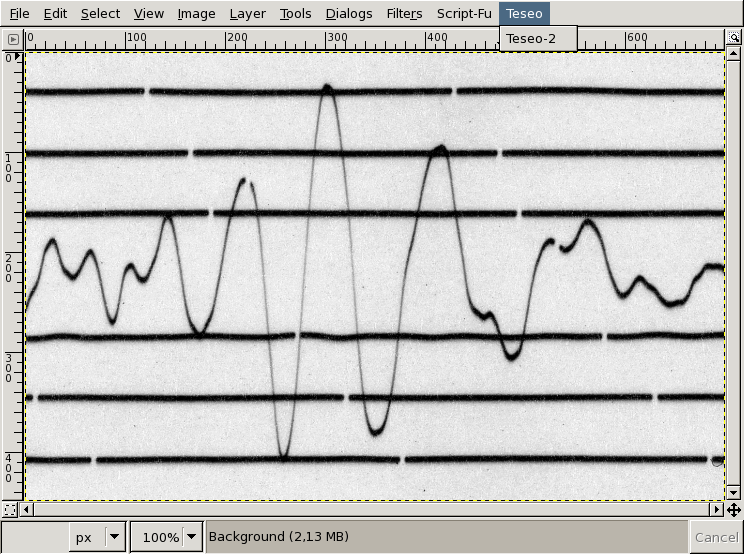
\includegraphics[width=10cm]{images/snapshot1.png}
\teseoincludegraphics{\teseoscalegraphics}{images/snapshot1.png}
\caption{Teseo menu}
\label{fig:teseomenu}
\end{center}
\end{figure}


\warning{When \teseo\ is launched, it is automatically \teseoquote{linked} to the image by the \gimp. We suggest to vectorize one image at a time and to respect the following order using \teseo: open image, open \teseo, close \teseo, close image. The name of the image is visible in the main window of \teseo.
If you close the image before \teseo, then close \teseo\ before reopening the image. Moreover, if you rename the image, \teseo\ work well but the references to the correct session are lost. In this case, we strongly recommend to open \teseo\ only after renaming the image.}

\warning{If \teseo\ crashes or \gimp\ is closed before \teseo, the session linked to the image remains locked. Next time you open \teseo\ on the same image, a warning message will be shown asking for forcing the session unlock. This mechanism is useful to prevent multiple instances of \teseo\ for the same image: only one instance for each image is allowed for a correct vectorization.}


\subsection{Session}

\teseo\ associates to the image some information related to seismogram paper, seismic event, station data and vectorization parameters. This information is saved in a \parolachiave{session} and it is referred to a single \parolachiave{seismic event}.

When you start  \teseo\ for the first time on an image, you are required to create a new session. Fill the fields shown in the figures \ref{fig:sessionrecord}, \ref{fig:sessiontraces}, \ref{fig:sessionpath}, and click \button{OK}.

Session properties can be modified at any time selecting File$\rightarrow$ Session$\rightarrow$ Properties (Ctrl+P in \teseo\ context). New sessions related to other events in the same image can be created selecting File$\rightarrow$ Session$\rightarrow$ New (Ctrl+N in \teseo\ context). The user can not change session file name because \teseo\ uses a fixed session naming convention.

Files related to the session are stored in \textsf{gimp\_directory}/{\itshape teseo--2}, where \textsf{gimp\_directory} is the user--specific \gimp\ settings directory. Usually, it is the subdirectory {\itshape .gimp--2.2} in the user home directory.

When \teseo\ is started on an image associated to more sessions, the user can choose the preferred one.
All the parameters described below are saved in the \parolachiave{session} file and, on demand, they can be imported or exported in \teseo\ \parolachiave{parasites} (section \ref{sec:teseoparasites}) and saved in the \xcf\ image.

\begin{figure}[!ht]
\begin{center}
% 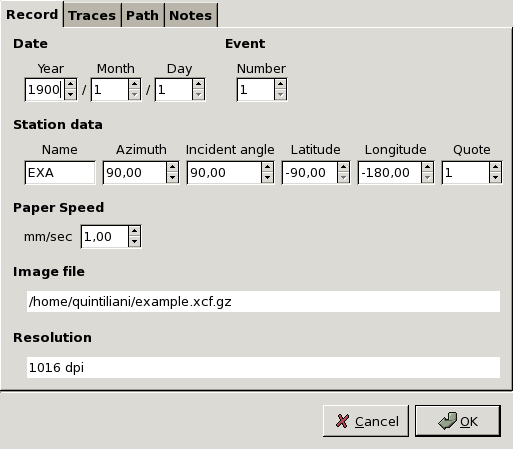
\includegraphics[width=10cm]{images/snapshot2.png}
\teseoincludegraphics{\teseoscalegraphics}{images/snapshot2.png}
\caption{Session window -- Record tab}
\label{fig:sessionrecord}
\end{center}
\end{figure}

In figure \ref{fig:sessionrecord} are shown the parameters associated to the seismic record.

\begin{itemize}
\item \parameter{Date}: date of recording.
\item \label{item:eventnumber} \parameter{Event number}: arbitrary ordinal number which identifies the event contained in the image. Use it to distinguish several events on the same image or date.
\item \parameter{Station data}: the following parameters will be saved in \fileformat{SAC} files.
	\begin{itemize}
	\item \parameter{Name}: station code.
	\item \parameter{Azimuth}: component azimuth (degrees clockwise from north).
	\item \parameter{Incident angle}: component incident angle (degrees from vertical).
	\item \parameter{Latitude}: station latitude (degrees, north positive).
	\item \parameter{Longitude}: station longitude (degrees, east positive).
	\item \parameter{Elevation}: station elevation (meters).
	\end{itemize}
\item \parameter{Paper speed}: linear velocity of the paper [mm/min].
\item \parameter{Image file}: name of the current image ({\itshape read-only}).
\item \parameter{Resolution}: image resolution ({\itshape read-only}).
\end{itemize}

\begin{figure}[!ht]
\begin{center}
% 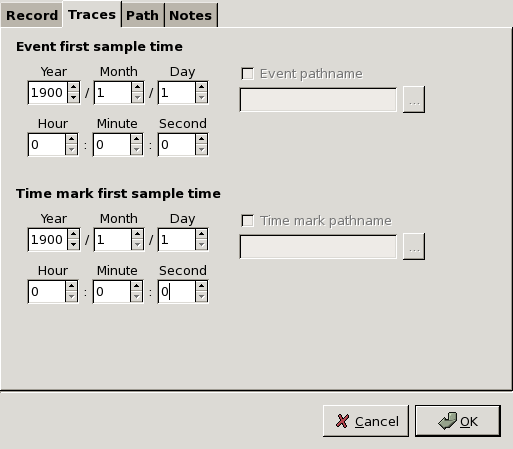
\includegraphics[width=10cm]{images/snapshot3.png}
\teseoincludegraphics{\teseoscalegraphics}{images/snapshot3.png}
\caption{Session window -- Traces tab}
\label{fig:sessiontraces}
\end{center}
\end{figure}

In figure \ref{fig:sessiontraces} are shown the parameters associated to the traces.

\begin{itemize}
\item \parameter{Event first sample time}: time of the first sample of the trace, this value will be saved in \fileformat{SAC} files.
\item \parameter{Time mark first sample time}:  time of the first sample of the trace that represents the time mark.
\end{itemize}


\begin{figure}[!ht]
\begin{center}
% 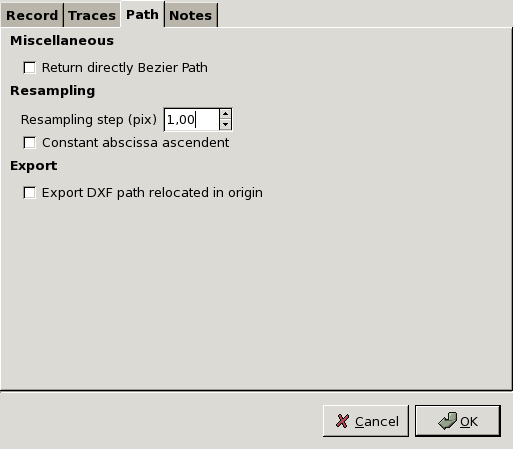
\includegraphics[width=10cm]{images/snapshot4.png}
\teseoincludegraphics{\teseoscalegraphics}{images/snapshot4.png}
\caption{Session window -- Path tab }
\label{fig:sessionpath}
\end{center}
\end{figure}

In figure \ref{fig:sessionpath} are shown the parameters associated to the path manipulation.

\begin{itemize}
\item \parameter{Return directly \beziername\ path}: if checked, when you use automatic vectorization methods, \teseooperations{Path Fit} is executed after every group of iterations.
\item \parameter{Resampling step}: samples are always evenly spaced with this distance in pixel.
\item \parameter{Constant abscissa ascendent}: if checked, X-values of the returned samples are strictly increasing, else X-values are evenly spaced regardless direction.
\item \parameter{Export DXF path relocated in origin}: if checked, \fileformat{DXF} export will translate the path starting a the coordinate (0, 0). This option is needed only for \sismos\ procedures.
\end{itemize}


\subsection{Teseo parasites}
\label{sec:teseoparasites}

In order to share and distribute results about the vectorization of a seismogram, \teseo\ includes all information related to the seismogram and his vectorization within a single file. This can be made using \gimp\ proprietary image format: the \xcf\ format.
In fact, \xcf\ format stores paths, layers, channels and \teseoquote{\parolachiave{parasites}},
a mechanism provided by \gimp\ for attaching arbitrary pieces of data to an image.

\teseo\ parasites contain all parameter values for the current session. When you import or export a session as parasites you have to consider the \parameter{Event number} (see figure \ref{fig:sessionrecord}). Remember that \parameter{Event number} is arbitrary and it could be thinked as the ordinal number associated to the sequence of the events occurred in the same \parameter{Date}. You can export only one set of the parameters for each single event.

Parasite operations are:

\begin{itemize}
	\item \teseooperations{Parasite Import}: import the n-th event contained in the \xcf\ image into the current \parolachiave{session}.
	\item \teseooperations{Parasite Export}: export all parameters of the current \parolachiave{session} into the \xcf\ image as parasite.
	\item \teseooperations{Parasite Remove all}: remove all \teseo\ \parolachiave{parasites} contained in the \xcf\ file.
\end{itemize}


\warning{When \parolachiave{parasites} related to an image are modified, remember to save the image before closing it. \gimp\ won't give you any advice before leaving the image.}



\section{Vectorization}

\teseo\ trace vectorization completely relies on \gimp\ \gimptool{Path} tool, which permits to create piecewise cubic \beziername\ curves and polygonals. Please, see \cite{gimphelp} for basic usage.

\warning{\teseo\ does not support closed paths.}

\warning{Seismogram must be oriented from left to right and top to bottom. If necessary you can use \gimp\ tools such as \gimptool{Flip} or \gimptool{Rotate} to modify the image ;-)}


\subsection{Multiple components in a path}
\label{sec:multiplecomponents}

\warning{Unfortunately, \gimp\ plug-in developers do not have yet available procedures (API) to handle paths with two or more components. \textbf{User must not create multiple components in a single path.}}

 If you accidentally generate a path containing multiple components you can combine them following these steps:

\begin{enumerate}
	\item Export the path in \fileformat{SVG} format using the \gimp\ Path Dialog.
	\item Import the path using the \teseo\ Menu File$\rightarrow$ Path$\rightarrow$ Import$\rightarrow$ SVG Combine. This procedure import the path and link sequentially the components each other.
	\item The previous steps could reverse the points order of the path. In this case use Path$\rightarrow$ Flip in the \teseo\ main window.
\end{enumerate}


\subsection{Manual}

You can manually vectorize the traces by \gimp\ \gimptool{Path} tool creating several piecewise cubic \beziername\ curves or polylines.

You should improve your manual dexterity before facing up to a complicated seismogram. Inside the distribution you find a very simple piece of seismogram to test your skill, the file name is {\itshape example.xcf.gz}. Keep in mind that the whole vectorization is based on \gimp\ \gimptool{Path} tool and it is wise to learn as much as possible about it.

{\itshape example.xcf.gz} contains a few paths manually made and others made by the \teseo\ colour weighted mean algorithm, which will be described in the next section \ref{subsec:automatic}.


\subsection{Automatic}
\label{subsec:automatic}

\teseo\ is designed to easily add algorithms for automatic seismogram vectorization.
An iterative procedure takes place whereby at each step the
algorithm is executed providing it with:
\begin{itemize}
\item a rectangular portion of the image centred at the last point of the current path;
\item information regarding the closest previous points;
\end{itemize}

in order to find the next point.

Presently, \teseo\ uses an algorithm based 
on a weighted mean of the trace colour (see subsection \ref{sec:cwm})

In future versions of \teseo\ more algorithms should be available (neural network approach too) and will be associated to other buttons beside \parolachiave{CWM} one.


In figure \ref{fig:teseogeneral} the main parameters of \teseo\ automatic path vectorization tool are shown:

\begin{itemize}
\item \parameter{Forward}: algorithm stop condition, maximum iteration number.
\item \parameter{Back}: number of points to delete from the current path.
\item \parameter{Stop to the first guide}: alternative stop condition, the iterations stop when the abscissa is greater than first vertical guide position.
\item \parameter{Trace colour}: base trace colour (black or white).
\item \parameter{Trace thickness}: thickness average in pixels.
\end{itemize}

The arrow buttons on the main window become sensitive when the user chooses an algorithm to execute.
To calculate the next point, the algorithm can use the additional information provided by the user who suggests a direction clicking on arrow buttons.


\subsubsection{Colour Weighted Mean}
\label{sec:cwm}

For detailed information about this algorithm read \cite{pintore}.

The colour weighted mean algorithm takes a rectangular region of the image having width and height specified in tab shown in figure \ref{fig:teseocwm} and centered into the last point of the current path.
This algorithm is activated clicking on the colour weighted mean button on the toolbar in figure \ref{fig:teseogeneral}.

The arrow buttons are available to suggest the direction.


\begin{figure}[!ht]
\begin{center}
% 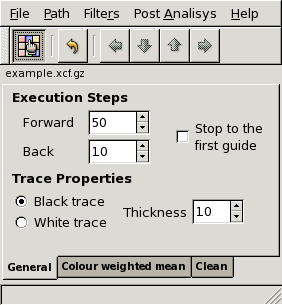
\includegraphics[width=7cm]{images/snapshot6.png}
\teseoincludegraphics{\teseoscalegraphics}{images/snapshot6.png}
\caption{Teseo window - General tab}
\label{fig:teseogeneral}
\end{center}
\end{figure}

\begin{figure}[!ht]
\begin{center}
% 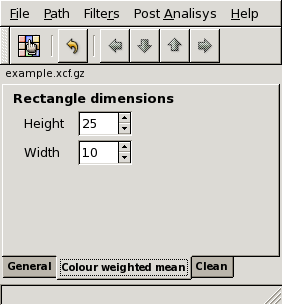
\includegraphics[width=7cm]{images/snapshot7.png}
\teseoincludegraphics{\teseoscalegraphics}{images/snapshot7.png}
\caption{Teseo window - Colour weighted mean tab}
\label{fig:teseocwm}
\end{center}
\end{figure}


\subsection{Path manipulation}

Besides \gimp\ \gimptool{Path} manipulation, \teseo\ adds some useful operations in seismogram vectorization.
In figure \ref{fig:teseopath} is shown the \teseo\ Path menu. The operations are subdivided in three groups: operations on the current path, operations on all unlocked paths and operations on path that represent Timemark.
Some operations rely on \gimp\ vertical guides tool: you can place a vertical guide clicking on the ruler on the left of the image window and
dragging it onto the image at the desired place.
\begin{itemize}
\item Current path operations
\begin{itemize}
	\item \teseooperations{Path Resample}: resample path with parameter defined in figure \ref{fig:sessionpath}.
	\item \teseooperations{Path Fit}: fit path with a piecewise cubic \beziername\ curve.
	\item \teseooperations{Path Split}:  split path at points defined by intersection beetwen path and \gimp\ vertical guides.
	\item \teseooperations{Path Force Polyline}: transform a path in a polyline. All the control points will be ignored.
        \item \teseooperations{Path Flip}: change the order of points in the selected path in the \gimp\ internal representation. Paths with the incorrect internal representation (with reversed order) could be created manipulating Paths with more than one component. Using them in \teseooperations{Align unlocked paths} and in {Link unlocked paths} give wrong results. Use \teseooperations{Path Flip} to restore correct points order.
	\item \teseooperations{Path Snap}: for each point compute a colour weighted mean in a thickness width square (figure \ref{fig:teseogeneral}).
\end{itemize}
\item Unlocked only paths operations
\begin{itemize}
	\item \teseooperations{Align unlocked paths}: align paths overlapping the first point of the next path to the last of the previous one.
This is the case when
the event is recorded over the paper margin and the trace lies on different lines.
This operation must be used before exporting the whole trace.
	\item \teseooperations{Link unlocked paths}: link paths with a straight line from the last point of the previous path to the first point of the next one. Useful to join several paths of the same event.
\end{itemize}
\item TimeMark
\begin{itemize}
	\item \teseooperations{Timemark - Evaluate intermediate TMs}: evaluate missing intermediate timemark of the current path and return vertical guides where they should be.
	\item \teseooperations{Timemark - Add TMs from guides}: add points where the guides intersect the current path.
\end{itemize}
\end{itemize}

\begin{figure}[!ht]
\begin{center}
% 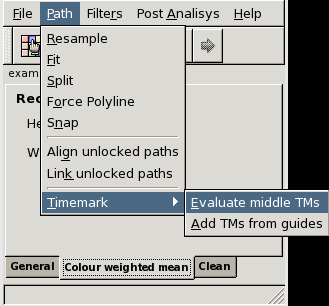
\includegraphics[width=7cm]{images/snapshot8.png}
\teseoincludegraphics{\teseoscalegraphics}{images/snapshot8.png}
\caption{Teseo window - Path menu}
\label{fig:teseopath}
\end{center}
\end{figure}


\warning{Order in operations on multiple paths respects order of the \gimp\ \gimptool{Path} tool, that is from bottom to top.
For example, executing a link on paths shown in figure \ref{fig:gimppathtool} results in a new path concatenating paths a, b and c in this order.}

\begin{figure}[!ht]
\begin{center}
% 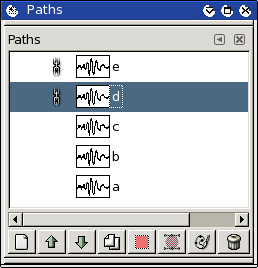
\includegraphics[width=7cm]{images/snapshot9.png}
\teseoincludegraphics{\teseoscalegraphics}{images/snapshot9.png}
\caption{\gimp\ Path Tool -- Path order}
\label{fig:gimppathtool}
\end{center}
\end{figure}
\vspace{0.5cm}



\subsection{Trace import/export}

\teseo\ imports and exports several file formats:

\begin{itemize}
        \item \fileformat{SVG}: Scalable Vector Graphics \cite{svg-spec}.
        \item \fileformat{DXF}: Drawing Interchange File Format \cite{adobe-dxf}.
        \item \fileformat{Trace}: \teseo\ proprietary ascii format. It contains image reference and coordinate in pixels. Only polylines.
        \item \fileformat{ASCII}: plain text file that contains the coordinates {\itshape (x,y)} sequence in millimeters. Only polylines.
        \item \fileformat{SAC}: Seismic Analysis Code \cite{goldstein}. Evenly spaced binary SAC. Only polylines.
        \item \fileformat{SISMA}: plain text file \teseoquote{Sismogrammi Storici} software compliant.
        \item \fileformat{Timemark}: plain text file that contains coordinates {\itshape (x,y)} sequence identifying timemarks.
        \item \fileformat{\beziername}: \gimp\ 1.0 \beziername\ path format. For downward compatibility.
        \item \fileformat{Examples}: binary format that contains information for neural networks learning. Not available yet.
\end{itemize}

Up to now, \fileformat{SVG} export is possible only by \gimp\ \gimptool{Path} tool, \fileformat{DXF} import is possible only on \teseo\ exported paths, \fileformat{SAC} import is not implemented yet.



\subsection{Filters}

\gimp\ offers a variety of filters and instruments to manipulate images. We strongly recommend to enhance the \teseoquote{readability} of your seismogram before vectorize. For example you could increase the contrast of the image.

\warning{If you want save the history of the changes applied to the image, you may apply the filters on copies of the \teseoquote{Background Layer}. Remember that all operations usually work on the current layer which could not necessarily be the visible one.}

At the moment, \teseo\ provides a graphical filter useful to \filter{clean} a seismogram.
What do we intend to clean a seismogram? Often, before vectorizing, it is advantageous to remove horizontal traces
crossing it while mantaining trace continuity. 
The main idea is to fill unwanted horizontal or vertical segments with the background color of the seismogram.

\warning{Good results are obtained when the noisy lines are perfectly horizontal. You can estimate required rotation using \gimp\ \gimptool{Measure} tool and then using \gimp\ \gimptool{Rotate} trasformation tool to rotate effectively. See \gimp\ help.}

In figure \ref{fig:teseofilterclean} it is possible to see the parameters related to the \filter{clean} filter.

\begin{figure}[!ht]
\begin{center}
% 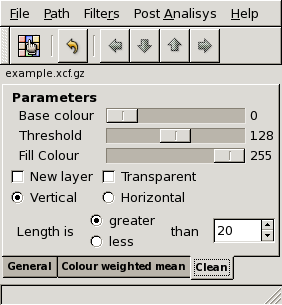
\includegraphics[width=7cm]{images/snapshot12.png}
\teseoincludegraphics{\teseoscalegraphics}{images/snapshot12.png}
\caption{Teseo Filter Clean}
\label{fig:teseofilterclean}
\end{center}
\end{figure}

\begin{itemize}
\item \parameter{Base colour}: is the base colour of the trace. Value from 0 (black) to 255 (white).
\item \parameter{Threshold}: is the maximum value of tolerance on base colour.
\item \parameter{Fill colour}: is the colour used to fill contiguous lines belonging to the colour condition.
\item \parameter{New layer}: if checked, the current layer will be copied and the filters will be run on the copy.
\item \parameter{Transparent}: if checked, only the filled lines will be displayed, rest of the image will be transparent. This works only on layer with alpha channel.
\item \parameter{Horizontal}/\parameter{Vertical}: choose one to fill horizontal or vertical line.
\item \parameter{Greater}/\parameter{Less}: choose one to fill lines longer or shorter than length.
\item \parameter{Length}: length of a single line on the image.
\end{itemize}

% \todo{ Typical use of this filter is to combine the parameter \parameter{Horizontal}  with \parameter{Greater} than a short length and \parameter{Vertical} with \parameter{Less} than a long length.}

If you've never used this filter you should try it on the example image contained in your \teseo\ distribution.
Follow these steps:

\begin{enumerate}
\item Open {\itshape example.xcf.gz}
\item Select the \teseoquote{Background} layer inside the \gimp\ Layer Dialog and apply the filter using the following parameters:
	\begin{itemize}
	\item \parameter{Base Colour} = 0
	\item \parameter{Threshold} = 128
	\item \parameter{Fill Colour} = 255
	\item \parameter{New layer} checked 
	\item \parameter{Transparent} uncheked 
	\item \parameter{Vertical} checked
	\item \parameter{Less} checked 
	\item \parameter{Length} = 9 
	\end{itemize}

\item A layer named \teseoquote{Background copy} will be created.

\item Select the \teseoquote{Background} layer and apply the filter using the following parameters:
	\begin{itemize}
	\item \parameter{Base Colour} = 0
	\item \parameter{Threshold} = 200
	\item \parameter{Fill Colour} = 255
	\item \parameter{New layer} checked 
	\item \parameter{Transparent} uncheked
	\item \parameter{Horizontal} checked
	\item \parameter{Greater} checked 
	\item \parameter{Length} = 28 
	\end{itemize}

\item A layer named \teseoquote{Background copy \#1} will be created.

\item Select the layer named \teseoquote{Background copy} and set the layer parameter \parameter{Mode} to Multiply.
\end{enumerate}

Nice! Isn't it?

An animation of this operation is available on \url{http://sismos.ingv.it/teseo/filters/}.


\section{Analysis after trace vectorization}

The seismogram curve on the image has to be corrected to become a seismic data with right amplitude and time.
There are many errors that could be introduced during the digitization procedure that must be taken into account.

\begin{itemize}
\item Rotation of the sheet during image scanning is a first error that can be easily removed using Gimp Rotation tool with the correct angle. 
\item To obtain data as a sequence of samples and corresponding time a scaling related to the paper speed is always needed.
\end{itemize}

Several different corrections have to be applied too in order to eliminate errors due to the recording system of the seismograph. 

\begin{itemize}
\item Instruments with photographic recording suffer from a trace distortion due to the spiral trend on the seismogram paper. This trend is further removable with other analysis instruments like SAC2000 \cite{goldstein}. This distorsion applies to all--mechanical recording systems too, like the Wiechert seismographs.
\item Mechanical recording systems suffer from a curvature of the seismic trace, worst in case of great amplitude signal, due to the finite arm lenght and finite radius of the cylinder bearing the smoked paper. To correct this kind of distortion, \teseo\ offers an instrument able to create a new path starting from a curved one. The algorithm used by \teseo\ is taken from Cadek \cite{cadek} , while the code we use was originally written in Fortran by A. Schlupp. The algorithm needs some parameters, for a few of them \teseo\ offers some other instruments to evaluate. 
These instruments are derived from \cite{schlupp}.
\end{itemize}

%Una volta prodotta la traccia vettorializzata, 

%Post--analysis of the digitized trace is currently limited to curvature correction.

\subsection{Curvature correction}

For semplicity we suppose that speed is a constant for the path segment we consider, otherwise we can subdivide path in segments at constant speed, for example from a time marker to the subsequent. Then we can correct the resulting paths one by one. 

\begin{figure}[!ht]
\begin{center}
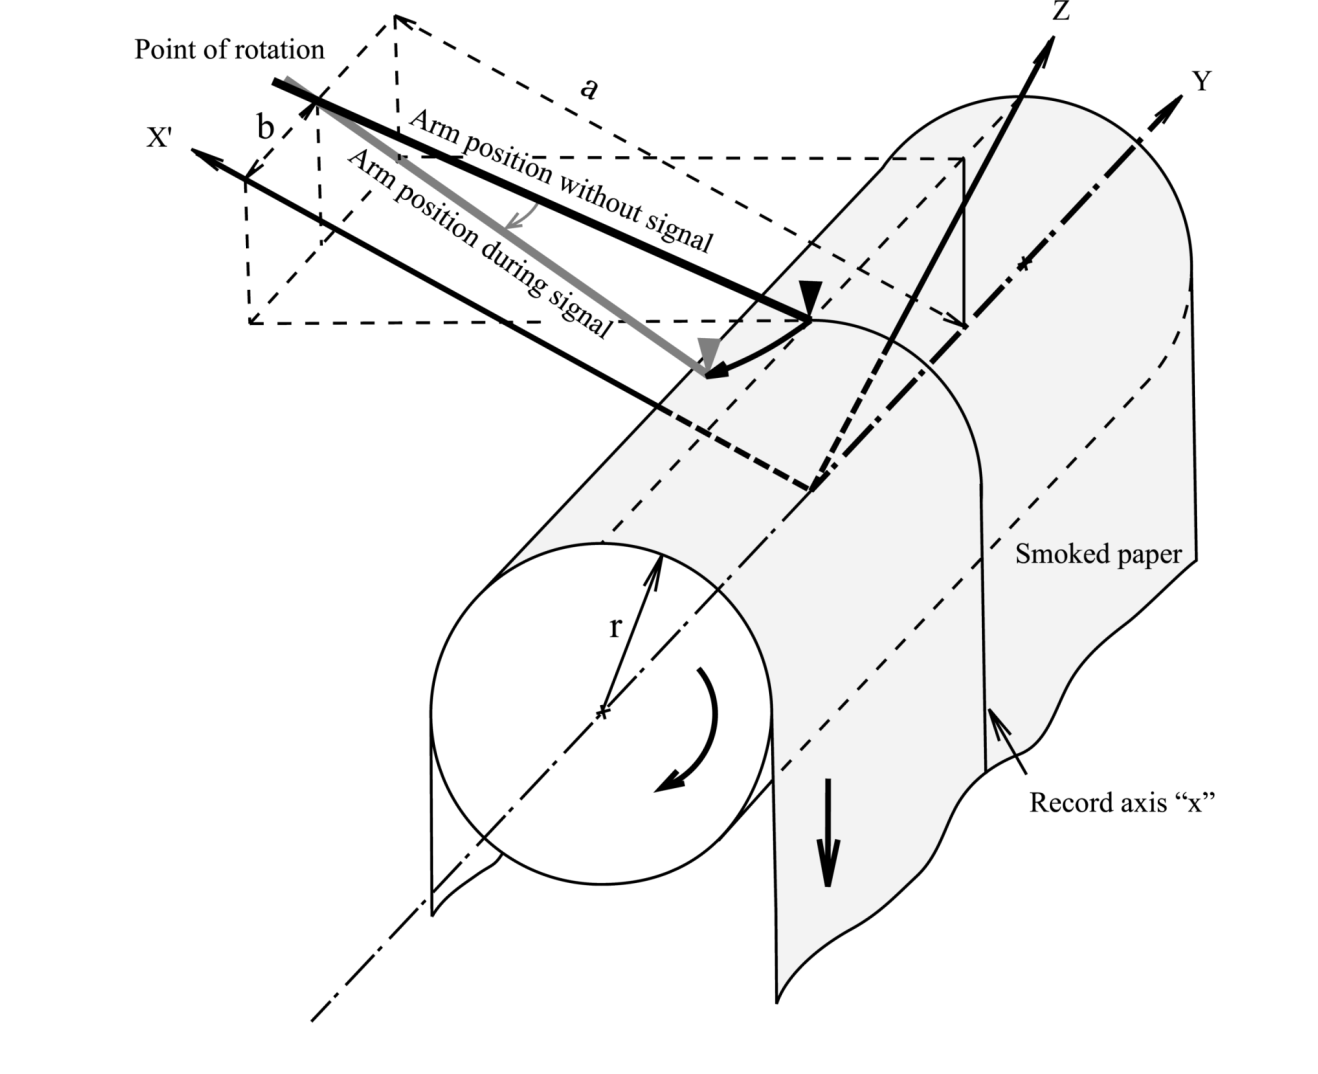
\includegraphics[width=14cm]{images/figure_III.2.png}
\caption{Mechanical recording schema.
{\itshape Figure provided by A. Schlupp.}
}
\label{fig:teseomrschema1}
\end{center}
\end{figure}

The formula for correction of the deformation due to the geometry of the recorder, as well as coordinate conversion (x,y) in time and amplitude, are given by Cadeck:

{\small
$$
t(i)= \frac{60}{d} \{ x(i) -r \frac{ arcsin \{ r^2+a^2 -R^2 +[y(i)-b]^2 \}}{ 2 a r } + r \frac{ arcsin ( r^2+a^2 -R^2 +b^2 )}{2 a r} \}
$$
}
%$$
%t(i)= \frac{60}{d} \{ B x(i) -r \frac{ arcsin \{r^2+a^2 -R^2 +[B y(i)-b]^2\}}{2 a r} + r \frac{arcsin [r^2+a^2 -R^2 +b^2]}{2 a r} \}
%$$

where:\\
\\
\parameter{R} = length of the writing arm, from its rotating axis to the tip of the needle \\
\parameter{r} = radius of the drive cylinder bearing the smoked paper\\
\parameter{a} = distance from the rotating arm axis to the driving cylinder axis \\
\parameter{b} = shift of the arm axis, in millimeters, to the base line on the smoked paper \\
\parameter{d} = minute length on the original record in millimeters \\
\parameter{x(i)} = coordinate to transform in seconds for time axis \\
\parameter{y(i)} = coordinate to transform in millimeters for amplitude axis \\
%\parameter{B} = conversion factor of x(i) coordinates, unknown unit, into millimeters (added to the original Cadeck formula) \\
%(Angles are in radians)


This formula applies to intruments modeled as in the schema shown in figure \ref{fig:teseomrschema1}.
To use this formula, it is necessary to get information about the seismogram.  For well known machinery, \parameter{r}, \parameter{R} and \parameter{a} can be retrieved from manufactory papers (figure \ref{fig:teseomrschema1}). Otherwise it is possible to adjust these parameters to reasonable values by trial and error. The \parameter{d} value is proportional to speed and resolution.

\begin{figure}[!ht]
\begin{center}
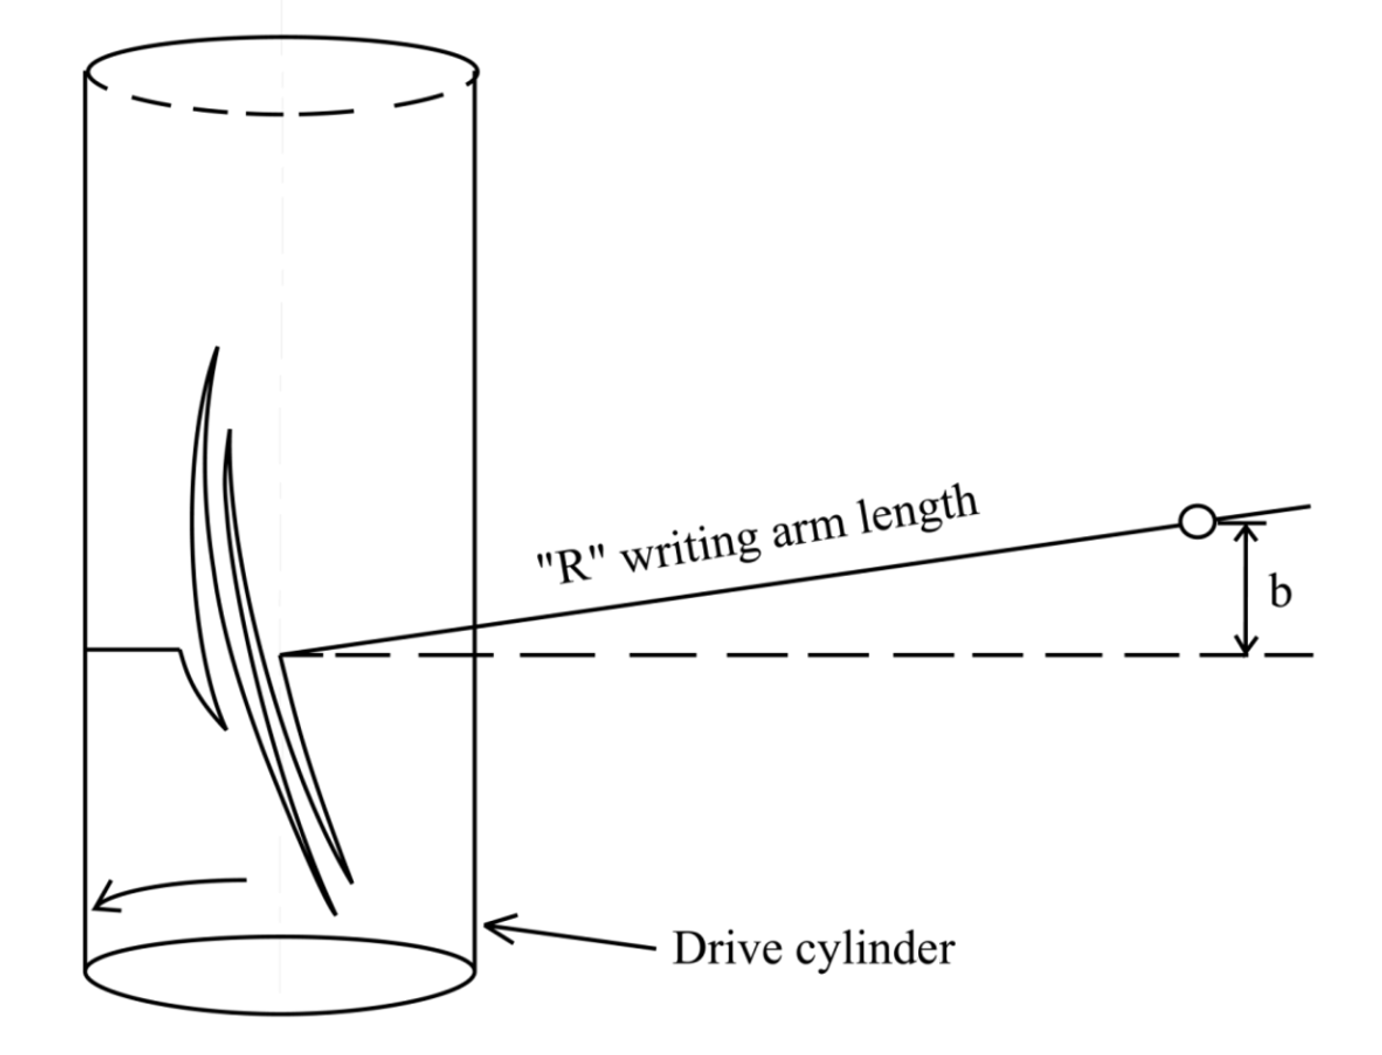
\includegraphics[width=14cm]{images/figure_III.3.png}
\caption{Mechanical recording schema: geometrical deformations induced by the shift \parameter{b} of the writing arm (after \cite{cadek}).
{\itshape Reproduced figure 3 \cite{schlupp}.}
}
\label{fig:teseomrschema2}
\end{center}
\end{figure}

The \parameter{b} value is the most difficult to determine and must be deduced directly from records, see figure \ref{fig:teseomrschema2}. A detailed description of the method to evaluate \parameter{b} is available in \cite{schlupp}.


\begin{figure}[!ht]
\begin{center}
\teseoincludegraphics{\teseoscalegraphics}{images/snapshot16.png}
\caption{Curvature Correction window}
\label{fig:teseocurvaturecorrection}
\end{center}
\end{figure}

Look at figure \ref{fig:teseocurvaturecorrection}, showing the  \menuname{Curvature Correction} window. You obtain this window clicking on \menuname{Curvature Correction} from \menuname{Post Analysis}. \\
%Clicking on \button{Correct} button you obtain a new path corrected applying the Cadeck formula with the parameters selected to the current path.\\
%Clicking on \button{Axial distance} button you obtain a calculation of \parameter{a} accordant to \parameter{r} and \parameter{R}, useful when \parameter{a} is unknown. \\
%Clicking on \button{Arm shift} button you obtain a plot of the various calculations of \parameter{b} and corresponding errors. You can choose the
%best \parameter{b}, presumably around the minimum of the function. The plot is interactive: you can zoom in selecting an area and clicking on the central mouse button. Right click to zoom out. Clicking on a point onto the plot select the abscissa of the point, the value is displayed in the Marked point field. \\
%Clicking on \parameter{Choose} you can save this value in the Arm shift field of the \menuname{Curvature Correction} window.\\
%Clicking on \button{Slopes} button you obtain a plot of the histogram of the slopes for the given \parameter{b}. According to \cite{schlupp} the histogram must be 0 or at his minimum at 90 degree for the correct Arm shift.


\begin{itemize}
\item {\bfseries Recorder geometry}
	\begin{itemize}
	\item \parameter{Arm length entry}: Enter the arm length value here.
	\item \parameter{Cylinder radius entry}: Enter the cylinder radius value here.
	\item \parameter{Axial distance entry}: Enter the axial distance value here.
	\item \button{Axial distance button}: Clicking on \button{Axial distance} button you obtain a calculation of \parameter{a} according to \parameter{r} and \parameter{R}, useful when \parameter{a} is unknown.
        \item \parameter{Arm shift entry}: Enter the arm shift value here.
	\item \button{Arm shift button}: Clicking on the \button{Arm Shift} button a "best" value of \parameter{b} will be calculated and showed in the \parameter{Arm shift entry}.
A plot of the error function calculated in a reasonable range of \parameter{b} will be shown: see figure \ref{fig:teseoberrors}.
	 You can choose an alternative \parameter{b} value, presumably around the minimum of the function. The plot is interactive: you can zoom in selecting an area and then clicking the central mouse button. Right click to zoom out. Click on a point in the plot to select the abscissa, the value is displayed in the Marked point field. Click on \parameter{Choose} to save it in the Arm shift entry.
	\end{itemize}
\item {\bfseries Record info}
	\begin{itemize}
	\item \parameter{Time span entry}: Time span from first to last point of the current path. Not required unless you select \parameter{Use time span}.
	\item \parameter{Paper velocity velocity}: Average speed of the paper for the current path. Required unless you select use \parameter{Time span}.
	\item \parameter{Lateral velocity}: Average lateral speed of the paper for the current path. Not required unless you select \parameter{Shift}
	\item \parameter{Scan rotation}: use it to compensate for a rotation introduced during the scanning phase -- angles are positive clockwise.  The correction is applied at the beginning of calculations. Not required unless you select \parameter{Rotate}
	\end{itemize}
\item {\bfseries Correction extrema} 
	\begin{itemize}
	\item \parameter{Starting X}: First point abscissa, not required unless you select \parameter{Use extrema}.
	\item \parameter{Starting Y}: First point ordinate, not required unless you select \parameter{Use extrema}.
	\item \parameter{Final X}: Last point abscissa, not required unless you select \parameter{Use extrema}.
	\item \parameter{Final Y}: Last point ordinate, not required unless you select \parameter{Use extrema}.
	\end{itemize}
\item {\bfseries Options}
	\begin{itemize}
	\item \parameter{Use extrema}: To use the user provided coordinates of the first and last point of the path. Useful for images with unknown  scale.
	\item \parameter{Use time span}: If you know exactly this time you can provide it to the algorithm. It will be used to calculate the speed.
	\item \parameter{Use raster angle}: To use the user provided error angle in scanning. If not checked the possible rotation angle will be calculated from the path.
	\item \parameter{Rotate}: Check to apply the rotation correction.
	\item \parameter{Shift}: Check to apply the lateral speed distortion correction.
	\end{itemize}
\item \button{Slopes} button: Click on \button{Slopes} button to plot the histogram of the slopes for the given \parameter{b}. According to \cite{schlupp} the slope should be $0$ or at his minimum at $90$ degree for the correct Arm shift.
\item \button{Correct} button: Click on \button{Correct} button to obtain a new path corrected applying the Cadeck formula with the parameters selected for the current path.
\end{itemize}


\begin{figure}[!ht]
\begin{center}
% 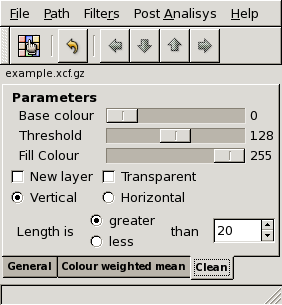
\includegraphics[width=7cm]{images/snapshot12.png}
\teseoincludegraphics{\teseoscalegraphics}{images/snapshot14.png}
\caption{Plot of the function Error(\parameter{b})}
\label{fig:teseoberrors}
\end{center}
\end{figure}

%Clicking on the \button{Arm Shift} button a "best" value of \parameter{b} will be calculated and showed in the box on the left of the button. A window will appear showing a plot of the \parameter{b}--Errors function see figure \ref{fig:teseoberrors} . User can then change the b value either manually after closing this window, or cliking on the choosen point then clicking on the \button{Choose} button in the window. 


\section{Before leaving Teseo}

Before closing \gimp\ is a very good practice to:

\begin{enumerate}
\item Save session (Ctrl+S in \teseo\ context)
\item Close \teseo.
\item Save \xcf\ file, it contains all your paths, layers and \teseo\ \parolachiave{parasites}. \xcf\ is your friend and gzip or bzip2 too.
\item Close \gimp.
\end{enumerate}



\section{Mailing list and bug report}

If you would like to:

\begin{itemize}
\item know news about \teseo
\item suggest further improvements
\item exchange experiences with others \teseo\ users
\item help the developers to improve \teseo\ and make it more stable
\end{itemize}

at the moment, the best way is subscribing the mailing list devoted to the \teseo\ users: feel free to send an e--mail to  \url{mailto:teseo-user-subscribe@yahoogroups.com} . However, the archive of the messages is open to everybody at \url{http://groups.yahoo.com/group/teseo-user/}


\subsection{Bug report}

\teseo\ is not a bug-free application, so if you find a bug, please report it sending an e--mail to \url{mailto:teseo@ingv.it} 

Please, remember to specify:
\begin{itemize}
\item Operating system
	\begin{itemize}
	\item {\small i.e.: Windows XP, Linux Distribution, Mac OS X version, ...}
	\end{itemize}
\item Teseo version
	\begin{itemize}
	\item {\small Teseo version looks like 2.x.x\\
	You find it in About window following Help$\rightarrow$ About in Teseo menu.}
	\end{itemize}
\item Kind of Teseo distribution
	\begin{itemize}
	\item {\small Source code, zip or tarball binaries, dmg image, ...}
	\end{itemize}
\item \gimp--2.2 version
	\begin{itemize}
	\item {\small \gimp\ version looks like 2.2.x}
	\end{itemize}
\item A detailed bug description
\end{itemize}

We will provide a bug tracking system if necessary.


\section{Credits}
\label{sec:credits}

\teseo\ source distribution contains code developed by other authors
and distributed respecting their copyright or license:

\begin{itemize}
\item {\bfseries Curvature correction} -- Curvature correction of Wiechert records is based on studies and Fortran routines developed by Antoine Schlupp. Within \teseo, Fortran routines have been ported in C.\\
	Author: {\itshape Antoine Schlupp} (\url{mailto:antoine.schlupp@eost.u-strasbg.fr})
\item {\bfseries NEWUOA} -- NEWUOA is a software developed by M.J.D. Powell for unconstrained optimization without derivatives.\\
	Author:  {\itshape M.J.D. Powell} (\url{mailto:mjdp@cam.ac.uk})
\item {\bfseries cfortran.h} -- cfortran.h is an easy-to-use powerful bridge between C and FORTRAN. It provides a transparent, machine independent interface between C and FORTRAN routines and global data. \url{http://www-zeus.desy.de/~burow/cfortran/}\\
	Author: {\itshape Burkhard Burow} (\url{mailto:burow@desy.de})
\end{itemize}


Main package dependencies are:

\begin{itemize}
\item {\bfseries GIMP} -- GNU Image Manipulation Program. \\
	\url{http://www.gimp.org/}
\item {\bfseries GtkDatabox} -- A Gtk+--Widget for Fast Data Display. \url{http://www.eudoxos.de/}\\
	Author:  {\itshape Roland Bock} (\url{mailto:rbock@eudoxos.de})
\end{itemize}


\section{Acknowledgements}

We would like to thank A. Schlupp for his contribution
in the Curvature Correction development.
We are also grateful to A. Michelini for his continuous encouragement
and to S. Mazza for his useful and constructive suggestions.


\listofwarnings

% \newpage
\listoffigures
% \lstlistoflistings
% \listoftables

% \nocite{*}
\bibliographystyle{apalike}
% \bibliographystyle{unsrt}
\newpage
\bibliography{Teseo2UserManual.bib}

\printindex
\end{document}


